\chapter{Roots and Integrals}

\section{Introduction}

In this lab, we will implement numerical alogirthms for root-finding
and integration.  We will apply the root finding algorithm to a
classic problem from quantum mechanics: the bound-state energy levels
of particle in finite potential well.  We will apply numerical
integration to the calculation of the periods of a simple pendulum.

For a faster but more challenging path, you can complete only the
problems (but including the optional challenges) in
Sections~\ref{sec:pbox} and \ref{sec:romberg}.

\section{Roots of a Linear Function}

It is usually best to start simple when developing code, so we'll develop our algorithms using a simple linear function with a root at $x=3$.\\

\plot Implement $f(x)=5\,(x-3)$ as a python function
\begin{python}
def f(x):
   # your code ...
\end{python}
Calculate the derivative of $f$ and implement it as the function:
\begin{python}
def fp(x):
   # your code ...
\end{python}
Check you code with:
\begin{python}
for x in [-1,3,4]:
    print(f(x), fp(x))
\end{python}
which should return:
\begin{verbatim}
-20 5
0 5
5 5
\end{verbatim}.

\section{Bisection Method}

In the bisection method, we start from values $a_1$ and $b_1$ where
$f(a_1) \cdot f(b_1) \leq 0$.  This condition insures that the range
$[a_1, b_1]$ contains at least one root.  The bisection method halves
the interval with each iteration, chosing the half that contains at
least one root.  Given $a_n$ and $b_n$, we calculate:
\begin{displaymath}
c_n = (a_n + b_n)/2
\end{displaymath}
we then determine:
\begin{displaymath}
a_{n+1}=
\begin{cases}
a_n & f(a_n) \cdot f(c_n) \leq 0 \\
c_n & \rm (otherwise) \\
\end{cases}
\end{displaymath}
and
\begin{displaymath}
b_{n+1}=
\begin{cases}
c_n & f(a_n) \cdot f(c_n) \leq 0\\
b_n & \rm (otherwise) \\
\end{cases}
\end{displaymath}

\plot Implement the python function
\begin{python}
def bisection(f, a, b):
   # your code  
   return a, b # updated values
\end{python}
which, given the function f=$f(x)$ and interval defined by a=$a_n$
b=$b_n$, returns the smaller interval defined by a=$a_{n+1}$ and
b=$b_{n+1}$ using the bisection algorithm.  Test your code with:
\begin{python}
print(bisection(f,0,4))
print(bisection(f,3,4))
\end{python}
which should have output:
\begin{verbatim}
(2.0, 4)
(3, 3.5)
\end{verbatim}

\section{Newton's Method}

We can use Newton's method to find the roots of a function $f(x)$ if we know its derivative $f'(x)$.
From our current best estimate for the root $x_n$ we calculate a better estimate as:
\begin{displaymath}
x_{n+1} = x_n - \frac{f(x_n)}{f'(x_n)}.
\end{displaymath}

\plot Implement the python function:
\begin{python}
def newton(f,fp,x):
    # your code
    return x # updated value
\end{python}
which, given the function f=$f(x)$, it's derivative fp=$f'(x)$, and the current best estimate for the root x=$x_n$, 
returns the improved estimate $x_{n+1}$.  Test your code as:
\begin{python}
for x in [-100,5,1000]:
   print(newton(f,fp,x))
\end{python}
which should return the values $3$, $3$, and $3$.  Why does one single iteration of Netwon's method find the root in this case?

\section{Secant Method}

When we do not know the derivative a function, we can use the secant
method.  The secant method provides an improved estimate for the root
$x_{n+1}$ from the previous two estimates $x_n$ and $x_n-1$ which are used to 
estimate the derivative and then apply Newton's method:

\begin{displaymath}
x_{n+1} = x_n - f(x_n) \frac{x_n-x_{n-1}}{f(x_n) - f(x_{n-1}}
\end{displaymath}\\

\plot Implement the python function:
\begin{python}
def secant(f,a,b):
   # your code here  
   return b,c  
\end{python}
which, given the function f=$f(x)$, and two previous estimates for the root a=$x_{n-1}$ and b=$x_n$, returns the updated estimates $b=x_n$ and $c=x_{n+1}$ using the secant method.  Test your code as:
\begin{python}
print(secant(f,0,4))
print(secant(f,5,3))
\end{python}
which should return
\begin{verbatim}
(4, 3.0)
(3, 3.0)
\end{verbatim}

\section{Roots of a Quadratic Function}

In this section, we will test your root finding algorithms on a quadratic equation:
\begin{equation}
  g(x) = (x-1) \, (x-4)
\end{equation}

\plot Define a python function \pyth{g(x)} which returns the value
$g(x)$.  Calculate the derivative $g'(x)$ analytically, and define
\pyth{gp(x)} which returns $g'(x)$.  Plot $g(x)$ and $g'(x)$ for
$0<x<5$.  Be sure to include axis labels and a legend. \\

\plot Apply five iterations of your function \pyth{bisection} to the range (0,2.5).  Do you approach the correct root?   \\

\plot  Starting from estimates a=0 and b=2.5, apply five iterations of your function \pyth{secant}.  Do you approach the correct root? \\


\plot Starting from the value x=2.5, apply five iterations of your function \pyth{newton}.  Do you approach a root? \\

\section{Particle in a Finite Potential Well}
\label{sec:pbox}

Suppose a particle of mass $m$ and energy $E$ is located in a finite potential well of form:
\begin{displaymath}
  V(x) =
  \begin{cases}
    V_0 & x \leq -L/2 \\
    0 & -L/2 < x < L/2 \\
    V_0 & L/2 \leq x \\
   \end{cases}
\end{displaymath}
We are going to consider the interesting situation where $E<V_0$, that
is, when the particle is bound by the potential.  For simplicity, we
will also assume the particle is in a symmetric state, such that wave
function $\psi$ has the property $\psi(-x)=\psi(x)$.  In this case, the
solutions to the Schrodinger Equation satisfy the transcendental
equation:
\begin{equation}
\label{eqn:transcendental}
v \tan v = \sqrt{v_0^2 - v^2}
\end{equation}
where 
\begin{displaymath}
v = L \sqrt{\frac{m \, E }{2 \hbar}}
\end{displaymath}
and
\begin{displaymath}
v_0^2 = \frac{m \, L^2 \, V_0}{2 \hbar} 
\end{displaymath}
are both dimensionless quantities, related to the particle energy $E$
and the potential energy of the well $V_0$.  If you haven't
yet encountered this essential problem from quantum mechanics, you can
just take my word about Equation~\ref{eqn:transcendental} for now.

\begin{figure}[htbp]
\begin{center}
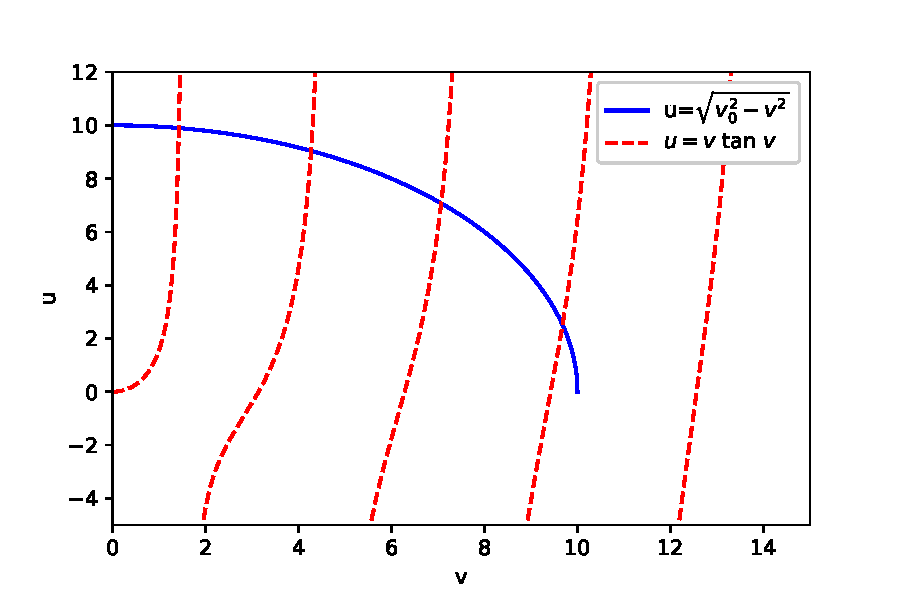
\includegraphics[width=0.65\textwidth]{figs/roots/transcendental.pdf} 
\caption{Graphical solution to Equation~\ref{eqn:transcendental} for $v_0=10$}
\label{fig:transcendental}
\end{center}
\end{figure}

Most quantum mechanical textbooks suggest that the solutions to
Equation~\ref{eqn:transcendental} may be obtained ``graphically'', by
plotting $u = v \tan v$ and $u = \sqrt{v_0^2 - v^2}$ and observing where
they intersect.  This approach is illustrated in
Fig.~\ref{fig:transcendental} for $v_0=10$.  You can see from the plot
that there are four places where these curves intersect.  In a
classical system, the particle could have any $E<V_0$, but in quantum
mechanical system, the particle may have only one of the four energy
values corresponding to the four intersection points. The number of
interesections, and where they occur, depends on the particular value
of $v_0$.\\

\plot Reproduce Fig.~\ref{fig:transcendental}. If you attempt to plot
the dashed red lines all at once, you will introduce
superflous vertical lines from when $\tan v$ switches from $+\infty$ to
$-\infty$.  To avoid this, plot each continuous region of $u = v \tan
v$ separately, in the regions $(-\pi/2,\pi/2)$, then $(\pi/2,3\pi/2)$,
and so on.  You may find it useful to remove problematic end points
from a numpy array by slicing them off like this \pyth{x=x[1:-1]}.
Instead of the math formulas, your legend may use the simpler labels LHS and RHS
, which refer to the left hand side and right hand side of
Equation~\ref{eqn:transcendental}.\\

Determining the bound state energy levels of quantum system is of
fundamental importance.  For just one example, we are able to
determine the chemical composition of stars using spectroscopy.  The
light frequencies which are readily absorbed by each element are
determined from the difference in the bound state energy levels.  In
this section, we will use numerical techniques to accurately determine
the values of $v$ which satisfy Equation~\ref{eqn:transcendental}.
This is equivalent to finding the bound-state energy levels.  We will
do so by finding the roots of the equation:
\begin{equation}
\label{eqn:hx}
h(x) = v \tan v - \sqrt{v_0^2 - v^2}
\end{equation}\\

\plot Define a function:
\begin{python}
def h(x):
   # your code   
\end{python}
which implements $h(x)$ from Equation~\ref{eqn:hx} for $v_0=10$.  Test it with:
\begin{python}
for v in [1,1.5,2,4.5]:
    print(np.around(h(v),2))
\end{python}
which should output the values -8.39, 11.27, -14.17, and 11.94.\\

\plot For $v_0=10$, determine the four roots of $h(x)$ using the bisection algorithm.\\

\plot For $v_0=10$, determine the four roots of $h(x)$ using the
secant algorithm.  To get reliable performance, you might want to
start by applying five iterations of the bisection algorithm.\\

\plot Calculate the derivative of $h(x)$ analytically, and implement it for $v_0=10$ as the python function \pyth{hp(x)}. Test you function as:
\begin{python}
for v in [1,1.5,2,4.5]:
    print(np.around(hp(v),2))
\end{python}
which should output the values 5.08, 314.03, 9.57, and 106.41.

\plot For $v_0=10$, determine the four roots of $h(x)$ using Newton's method. \\

\plot (Optional Challenge) The antisymmetric solutions to the Schrodinger Equation satisfy the equation:
\begin{displaymath}
- v \cot v = \sqrt{v_0^2 - v^2}
\end{displaymath}
Find the solutions for $v$ using Newton's method.\\

\plot (Optional Challenge) The Wikipedia article on the finite potential well lists the solutions to $v$ for $v_0^2=20$.  Verify their results.

\section{Trapezoid Method}

The trapezoid method approximates the definite integral
\begin{displaymath}
I = \int_a^b f(x) \, dx
\end{displaymath}
from the function evaluated at $n$ evenly spaced points
\begin{displaymath}
I_T =  \frac{h}{2}(f(a) + f(b)) + h \, \sum_{i=1}^{n-1} f(x_i)
\end{displaymath}
where
\begin{displaymath}
h = \frac{b-a}{n-1}
\end{displaymath}
and
\begin{displaymath}
x_i = a + h \, i 
\end{displaymath}
The truncation error is:
\begin{displaymath}
I-I_T = \mathcal{O}(h^2).
\end{displaymath}
Notice that the sum is over the interior points, which have twice the
weight of the end points at $a$ and $b$.

\plot Implement the python function:
\begin{python}
def trapezoid(f,a,b,n):
   # your code
   return sum
\end{python}
Which returns the integral of f=$f(x)$ from a to b, using the
trapezoid method from $n$ evenly spaced points.
Test your code with:
\begin{python}
print(np.around(trapz(np.sin,0,np.pi/2,2),2))
print(np.around(trapz(np.sin,0,np.pi/2,3),2))
print(np.around(trapz(np.sin,0,np.pi/2,4),2))
\end{python}
which should output the values 2.36, 1.73, and 1.5.

\section{Iterative Trapezoid Method}

In the iterative trapezoid method, we halve the spaces between points
during each interation, so that:
\begin{displaymath}
h_1 = (b-a), \; h_2 = \frac{b-a}{2}, \; \ldots \; , \; h_m = \frac{b-a}{2^{m-1}}
\end{displaymath}
Because the interval size $h_{m+1}$ is one half the previous interval
$h_m$, we can avoid evaluating previously evaluated $x$ values by
resusing the previous iteration:
\begin{displaymath}
I_{m+1} = \frac{1}{2} \, I_{m} + h_{m+1}\sum_{i=1}^{2^{(m-1)}} f(a+(2i-1)h_{m+1}).
\end{displaymath}
Take care when reading that the upper limit on the sum is $2^{(m-1)}$
not $2\,(m-1)$.  A major benefit of this approach is that the
difference between $I_{m+1}$ and $I_m$ can be used to estimate the
truncation error.\\

\plot Implement the python function:
\begin{python}
def itertrap(f,a,b,s,m):
   # your code
   return s, m # updated values! 
\end{python}
Which calculates one iteration of the iterative trapezoid method for
the integral of f=$f(x)$ from a to b, starting from s=$I_{m}$. Returns
the updated values $\rm{s} \to I_{m+1}$ and $\rm{m} \to m+1$.
Test your code with:
\begin{python}
print(np.around(itertrap(np.sin,np.pi/2,np.pi,0.00,1),2))
print(np.around(itertrap(np.sin,np.pi/2,np.pi,0.56,2),2))
print(np.around(itertrap(np.sin,np.pi/2,np.pi,0.79,3),2))
\end{python}
which should output:
\begin{verbatim}
[0.56 2.  ]
[0.79 3.  ]
[0.9 4. ]
\end{verbatim}

\plot Calculate the definite integral:
\begin{displaymath}
I = \int_0^\pi \sin(x) \, dx
\end{displaymath}
using the iterative trapezoid method.  Notice that $I_1 = 0$ so start things off with $s=0$ and $m=1$.  Use the update idiom:
\begin{python}
s,m = itertrap(f, a, b, s, m)
\end{python}
and iterate until the estimated truncation error is less than $\sigma=10^{-6}$.


\section{Period of a Pendulum}

In this section we will consider the oscillation of a pendulum of length $L$ in a graviational field with magnitude $g$.  For small angles, the period of a pendulum oscillation is approximately a constant value:
\begin{displaymath}
T_0 = 2\pi \frac{L}{g}
\end{displaymath}
For oscillations at larger angles, the period of the oscillation cannot be calculated analytically. However, it can be expressed as a definite integral:
\begin{equation}
\label{eqn:elliptic}
\frac{T}{T_0} = \frac{2}{\pi}\int_0^{\pi/2}\frac{1}{\sqrt{1-k^2\sin u}}\,du 
\end{equation}
where:
\begin{displaymath}
k = \sin \frac{\theta_0}{2}
\end{displaymath}

\plot Estimate the ratio $T/T_0$ for $\theta_0=1$ using the iterative
trapezoid rule.  Iterate until the estimated truncation error is less
than $10^{-6}$.  Note that in this case $I_1$ is not zero, so you will
have to calculate the starting value for $s$.

\section{Romberg Integration}
\label{sec:romberg}

The section contains a challenging problem which will only represent a
small part of your grade (unless you have opted to take the fast and
challenging path.)  You should attempt to tackle if for yourself.
Your instructors will not help you solve this problem!  You should be
able to tackle this problem if you break it into steps and test each
step carefully, using all of the techniques you have learned this
quarter.  Don't be discourage if you cannot comnplete it successfully,
this is meant to be a challenge!

The Romberg Method is an ingenious approach to integration which
combines the iterative trapezoid rule with Richardson appoximation.
This is an example of a high-end algorithm which converges extremely
rapidly.  The method iteratively constructs the matrix $R$
\begin{displaymath}
\begin{pmatrix}
R_{1,1} &         &         &         & \\
R_{2,1} & R_{2,2} &         &         & \\
R_{3,1} & R_{3,2} & R_{3,3} &         & \\
\vdots  & \vdots  & \vdots  & \ddots  & \\
R_{m,1} & R_{m,2} & R_{m,3} & \cdots  & R_{m,m} \\
\end{pmatrix}
\end{displaymath}
The values in the leftmost column are constructed using the iterative trapezoid method:
\begin{displaymath}
R_{m,1} = I_m  
\end{displaymath}
and the entries to the right are calculated iteratively using Richardson's approximation:
\begin{displaymath}
R_{m,j+1} = \frac{4^j R_{m,j} - R_{m-1,j}}{4^j-1} 
\end{displaymath}
The best estimates are the values along the diagonal.

Note that each row is calculated using only values from previous row, so we will tackle this problem row by row.
Given:
\begin{displaymath}
\begin{pmatrix}
R_{1,1} \\
\end{pmatrix}
\end{displaymath}
the next iteration should return:
\begin{displaymath}
\begin{pmatrix}
R_{2,1} & R_{2,2} \\
\end{pmatrix}
\end{displaymath}
and given:
\begin{displaymath}
\begin{pmatrix}
R_{2,1} & R_{2,2} \\
\end{pmatrix}
\end{displaymath}
the next iterations should return:
\begin{displaymath}
\begin{pmatrix}
R_{3,1} & R_{3,2} & R_{3,3}\\
\end{pmatrix}
\end{displaymath}

\newpage

\plot (Challenging, not optional) Define  python function
\begin{python}
def romberg(f,a,b,R):
   # your code
   return R # updated value
\end{python}
which given the $m$th row as array R:
\begin{displaymath}
R = 
\begin{pmatrix}
R_{m,1} & R_{m,2} & \cdots & R_{m,m}\\
\end{pmatrix}
\end{displaymath}
returns the updated array:
\begin{displaymath}
R = 
\begin{pmatrix}
R_{m+1,1} & R_{m+1,2} & \cdots & R_{m+1,m+1}\\
\end{pmatrix}
\end{displaymath}
Test your code by calculating the definite integral:
\begin{displaymath}
I = \int_0^\pi \sin(x) \, dx
\end{displaymath}
by constructing four rows of the Romberg matrix.\\

\plot (Challenging, optional) Use Romberg integration to calculate the
period of a pendulum with length $L$ in a gravitational field of
strength $g$ which comes to rest at $\theta = \theta_0$, by
numerically integrating Equation~\ref{eqn:elliptic} using the Romberg
method.  Stop for a truncation error less than $10^{-6}$.
